\documentclass[12pt,a4paper]{report}
\usepackage[margin=2.54cm]{geometry}
\usepackage[T1]{fontenc}
\usepackage[utf8]{inputenc}
\usepackage{lmodern}
\usepackage{microtype}
\usepackage{graphicx}
\usepackage{booktabs}
\usepackage{longtable}
\usepackage{array}
\usepackage{tabularx}
\usepackage{threeparttable}
\usepackage{amsmath}
\usepackage{enumitem}
\usepackage[hidelinks]{hyperref}
\usepackage{csquotes}
\usepackage[backend=biber,style=authoryear,sorting=nyt]{biblatex}
\addbibresource{kampala_air_quality_thesis_chapter.bib}

\newcommand{\pmfive}{PM$_{2.5}$}
\newcommand{\ugm}{\ensuremath{\mu}\,g/m$^3$}
\newcommand{\placeholder}[1]{\textit{[#1]}}
\setlength{\emergencystretch}{3em}

\begin{document}

\begin{titlepage}
\centering
\vspace*{2cm}
{\Large \placeholder{University name} \par}
\vspace{1.5cm}
{\Large\bfseries Air Pollution and Respiratory Morbidity in Kampala, Uganda:\\
An Ecological Time-Series Analysis of Weekly Routine Surveillance Data\par}
\vspace{1.5cm}
{\large A thesis chapter submitted in partial fulfilment of the requirements for the degree of \placeholder{PhD degree}\par}
\vspace{1.5cm}
{\large \placeholder{Author name}\par}
\vfill
{\large Supervisors: \placeholder{Supervisor name(s)}\par}
\vspace{0.7cm}
{\large \placeholder{Department and university}\par}
\vspace{0.7cm}
{\large \placeholder{Month Year}\par}
\end{titlepage}

\pagenumbering{roman}
\chapter*{Abstract}
\addcontentsline{toc}{chapter}{Abstract}
\noindent\textbf{Background.} Fine particulate air pollution is an important environmental health concern, but evidence based on routinely collected morbidity data in East African cities remains limited. This chapter examined weekly associations between ambient \pmfive{} concentrations and four respiratory outcomes in Kampala, Uganda.\\
\noindent\textbf{Methods.} We linked weekly climate, averaged \pmfive{}, and routine respiratory surveillance records. The original primary analysis used 248 weeks through 15 December 2024; a harmonised sensitivity pipeline retained 262 weekly environmental records through 5 January 2025 and did not impute missing outcome counts. We additionally analysed 5,006 eligible medical-record-review observations from 2020--2024 by division, sex, age band, diagnosis, and same-day division-level monitored \pmfive{}. Count models and diagnosis case-mix models were adjusted for available temporal, demographic, and facility variables.\\
\noindent\textbf{Results.} The original primary model associated a 10 \ugm{} higher \pmfive{} concentration with higher ILI notifications (IRR 1.173, 95\% CI 1.030--1.335), whereas SARI and under-five pneumonia estimates were imprecise and the inverse TB estimate was not interpreted as protective. In the harmonised weekly lag analysis, ILI was higher at one-week lag (IRR 1.327, 1.086--1.621); results varied by lag and outcome. Of the medical-review records, 3,632 had same-day division-level exposure assignment. Within-division \pmfive{} associations with recorded ILI, pneumonia, SARI, and TB rates were imprecise or near null; the diagnosis case-mix analysis nevertheless showed higher odds of ILI versus other reviewed respiratory diagnoses (OR 1.749, 1.490--2.053).\\
\noindent\textbf{Conclusions.} Routine data revealed an outcome-specific association between \pmfive{} and ILI, but the ecological design, incomplete control of confounding, exposure aggregation, and surveillance artifacts preclude causal attribution. The findings support improved integrated environmental and health surveillance and prospective, pre-specified studies.

\vspace{0.5cm}
\noindent\textbf{Keywords:} particulate matter; air pollution; respiratory infection; routine surveillance; time series; Kampala; Uganda; ecological epidemiology.

\chapter*{Abbreviations}
\addcontentsline{toc}{chapter}{Abbreviations}
\begin{tabular}{ll}
\pmfive{} & Particulate matter with aerodynamic diameter $\leq 2.5\,\mu$m \\
CI & Confidence interval \\
ILI & Influenza-like illness \\
IRR & Incidence rate ratio \\
SARI & Severe acute respiratory infection \\
TB & Tuberculosis \\
\end{tabular}

\tableofcontents
\clearpage
\pagenumbering{arabic}

\chapter{Introduction}
\section{Background and rationale}
Ambient particulate matter is a policy-relevant exposure because inhalable particles can reach the lower respiratory tract and are linked to a wide range of adverse health outcomes. The World Health Organization (WHO) provides health-based guideline levels and interim targets for \pmfive{} and other pollutants \parencite{WHO2021}. Kampala faces traffic, road dust, combustion, and urban-development pressures that make local, decision-relevant evidence important. Yet a city-wide association estimated from routine data must be interpreted cautiously: notification counts reflect disease occurrence, care seeking, diagnostics, reporting, and health-service disruptions as well as environmental conditions.

This chapter uses project-supplied weekly records to examine whether variation in ambient \pmfive{} coincided with variation in four respiratory morbidity outcomes. It follows observational-reporting principles in the STROBE statement \parencite{vonElm2007} and separates association estimates from causal and policy claims.

\section{Research questions and objectives}
The primary research question was: \emph{How were weekly ambient \pmfive{} concentrations associated with weekly notifications of TB, ILI, severe pneumonia in children under five, and SARI in Kampala?}

The objectives were to: (i) describe the time series and seasonal patterns; (ii) estimate adjusted contemporaneous associations; (iii) examine 0--4-week lagged associations; (iv) test the stability of estimates in prespecified sensitivity analyses; and (v) describe division-level variation in available monitoring, medical-review, sex, age, and population data.

\section{Conceptual framework}
\begin{figure}[htbp]
\centering
\fbox{\parbox{0.88\textwidth}{\centering
\textbf{Emission sources and urban activity} (traffic, dust, combustion) $\rightarrow$
\textbf{ambient \pmfive{}} $\rightarrow$ \textbf{respiratory susceptibility, symptoms, and illness} $\rightarrow$
\textbf{health-care attendance, diagnosis, and notification}.\\[0.5em]
Temperature, humidity, precipitation, seasonality, secular trends, health-service access, diagnostic practice, and reporting completeness may affect both exposure patterns and notified morbidity.}}
\caption{Analytic conceptual framework. The routinely collected outcome is a notification count, not a direct measure of disease incidence.}
\label{fig:framework}
\end{figure}

\chapter{Methods}
\section{Design, setting, and analytic period}
This was an ecological weekly time-series analysis in Kampala, Uganda. The analytic period covered 5 January 2020 through 15 December 2024 and contained 248 reporting weeks. The unit of analysis was the calendar week; therefore, individual-level causation cannot be inferred from the study estimates.

\section{Data sources and linkage}
Three project-supplied sources were linked by epidemiological year and week or by the weekly ending date: (i) respiratory surveillance records, (ii) climate records containing temperature, humidity, wind speed, and precipitation, and (iii) weekly averaged \pmfive{} observations. The analytic dataset was constructed in \texttt{analysis\_no\_deaths.ipynb}; its provenance and source files are documented as project data \parencite{ProjectData2026}. The spatial analysis additionally used two supplied monitor-export files, a Kampala administrative-boundary shapefile, the medical-record abstraction workbook, and parish/division population counts.

All mortality fields were excluded before analysis. The four retained outcomes were: Pulmonary TB cases (TB), ILI cases, severe pneumonia under five cases, and SARI cases. Counts were modeled as supplied; no population denominators or offsets were available, so results describe associations with notified counts rather than incidence rates in the population.

\section{Data processing and feature construction}
Weekly dates were converted to dates, and duplicate climate/air-quality keys were reconciled during the merge. The legacy primary pipeline mean-imputed selected environmental and outcome fields. The harmonised sensitivity pipeline instead averaged duplicate environmental week records and retained missing outcome counts as missing; models used their available complete observations. The resulting series had 11 missing calendar weeks according to the processor log, so the time scale represents observed reporting weeks rather than an uninterrupted daily exposure series.

For exploratory analyses, the notebook generated 1--4-week \pmfive{} lags, rolling averages, outcome changes, temperature--humidity interactions, and rolling weather summaries. These features were used for descriptive and exploratory analyses; they were not all entered simultaneously in the primary regression.

\section{Primary statistical model}
For outcome $Y_t$ at week $t$, the primary Poisson generalized linear model was
\[
\log\{E(Y_t)\}=\beta_0+\beta_1\mathrm{PM}_{2.5,t}+\beta_2T_t+\beta_3H_t+\beta_4P_t+\beta_5\mathrm{month}_t+\beta_6t.
\]
The model included ambient \pmfive{}, temperature ($T$), relative humidity ($H$), precipitation ($P$), calendar month, and linear time. Robust HC3 standard errors were used. Estimates are expressed as $\exp(10\beta_1)$, the IRR associated with a 10 \ugm{} higher weekly \pmfive{} concentration. Poisson regression is a standard framework for count outcomes, while valid inference depends on appropriate mean specification and variance handling \parencite{CameronTrivedi2013}.

\section{Secondary and sensitivity analyses}
An exploratory distributed-lag model entered separate linear \pmfive{} terms at lags 0--4 weeks, adjusted for the same weather, month, and time terms. Lag-specific coefficients were summed with their covariance matrix to calculate a cumulative 0--4-week IRR. This simplified linear-lag specification is related to, but not a full implementation of, a distributed lag non-linear model \parencite{Gasparrini2010}.

Climate models reported temperature per 1$^\circ$C and relative humidity per 10 percentage-point increment. Sensitivity analyses (a) excluded the highest 5\% of \pmfive{} weeks and (b) replaced contemporaneous \pmfive{} with a one-week lag. The harmonised weekly and monthly sensitivity models used negative-binomial regressions with separate \pmfive{} lags (0--4 weeks and 0--2 months, respectively), calendar month, linear time, and available weather covariates.

For the medical-record analysis, records with valid Kampala division and visit date from 2020--2024 were retained. Exact or reviewed parish-name linkage to the population file succeeded for 2,425 of 5,006 records; this linkage was used for quality reporting, not to infer unmatched locations. Daily monitor readings were averaged within division and assigned on the visit day; 3,632 records had same-day exposure assignment. Division--time--sex--age--diagnosis counts were modelled with approximate sex--age population offsets derived from the available marginal denominators. \pmfive{} was decomposed into division mean and within-division deviation, following the group-mean-centering principle used in spatial air-pollution analyses \parencite{Adjorlolo2026}. Secondary logistic case-mix models compared each diagnosis with all other reviewed respiratory diagnoses, adjusted for sex, age band, month, facility, and \pmfive{}. These are associations with recorded cases, not population incidence or individual RTI risk.

\section{Exploratory predictive and intervention analyses}
The notebook also fitted LSTM-based models with an eight-week sequence, a nominal 80/20 temporal split, and environmental/time features. It benchmarked classical classifiers separately. A midpoint date of 29 May 2022 was mechanically designated as an intervention reference, not an observed policy intervention. Scenario calculations applied a fixed assumed relative risk of 1.08 per 10 \ugm{} change to hypothesized \pmfive{} reductions. These analyses are presented in Appendix~\ref{app:exploratory}; they were not used to support the principal epidemiological conclusions.

\chapter{Results}
\section{Analytic dataset}
The analytic series included 248 weeks. Mean \pmfive{} was 39.28 \ugm{} (SD 11.81; range 16.87--90.92). Mean weekly notified counts were 638.26 for TB, 339.95 for ILI, 124.11 for severe pneumonia in children under five, and 220.12 for SARI (Table~\ref{tab:descriptive}). ILI showed substantially greater relative variability than the other outcomes, consistent with episodic reporting or disease peaks.

\begin{table}[htbp]
\centering
\caption{Descriptive statistics for weekly analytic variables, Kampala, 2020--2024.}
\label{tab:descriptive}
\begin{tabular}{lrrrrr}
\toprule
Variable & Mean & SD & Minimum & Median & Maximum \\
\midrule
\pmfive{} (\ugm{}) & 39.28 & 11.81 & 16.87 & 38.06 & 90.92 \\
Temperature ($^\circ$C) & 22.85 & 0.97 & 20.83 & 22.72 & 27.04 \\
Relative humidity (\%) & 80.96 & 5.05 & 54.71 & 81.60 & 90.06 \\
Precipitation (mm/day) & 28.21 & 27.76 & 0.02 & 19.16 & 133.74 \\
TB cases & 638.26 & 251.80 & 7 & 638.26 & 1321 \\
ILI cases & 339.95 & 718.62 & 1 & 40.50 & 3498 \\
Severe pneumonia, under 5 & 124.11 & 75.61 & 4 & 116.00 & 1037 \\
SARI cases & 220.12 & 161.49 & 1 & 172.50 & 1375 \\
\bottomrule
\end{tabular}
\end{table}

Figure~\ref{fig:timeseries} shows co-occurring temporal variation in pollution and notified morbidity. The series are heterogeneous in scale and temporal shape; visual co-movement alone does not distinguish pollution effects from seasonal or reporting processes.
\begin{figure}[htbp]
\centering
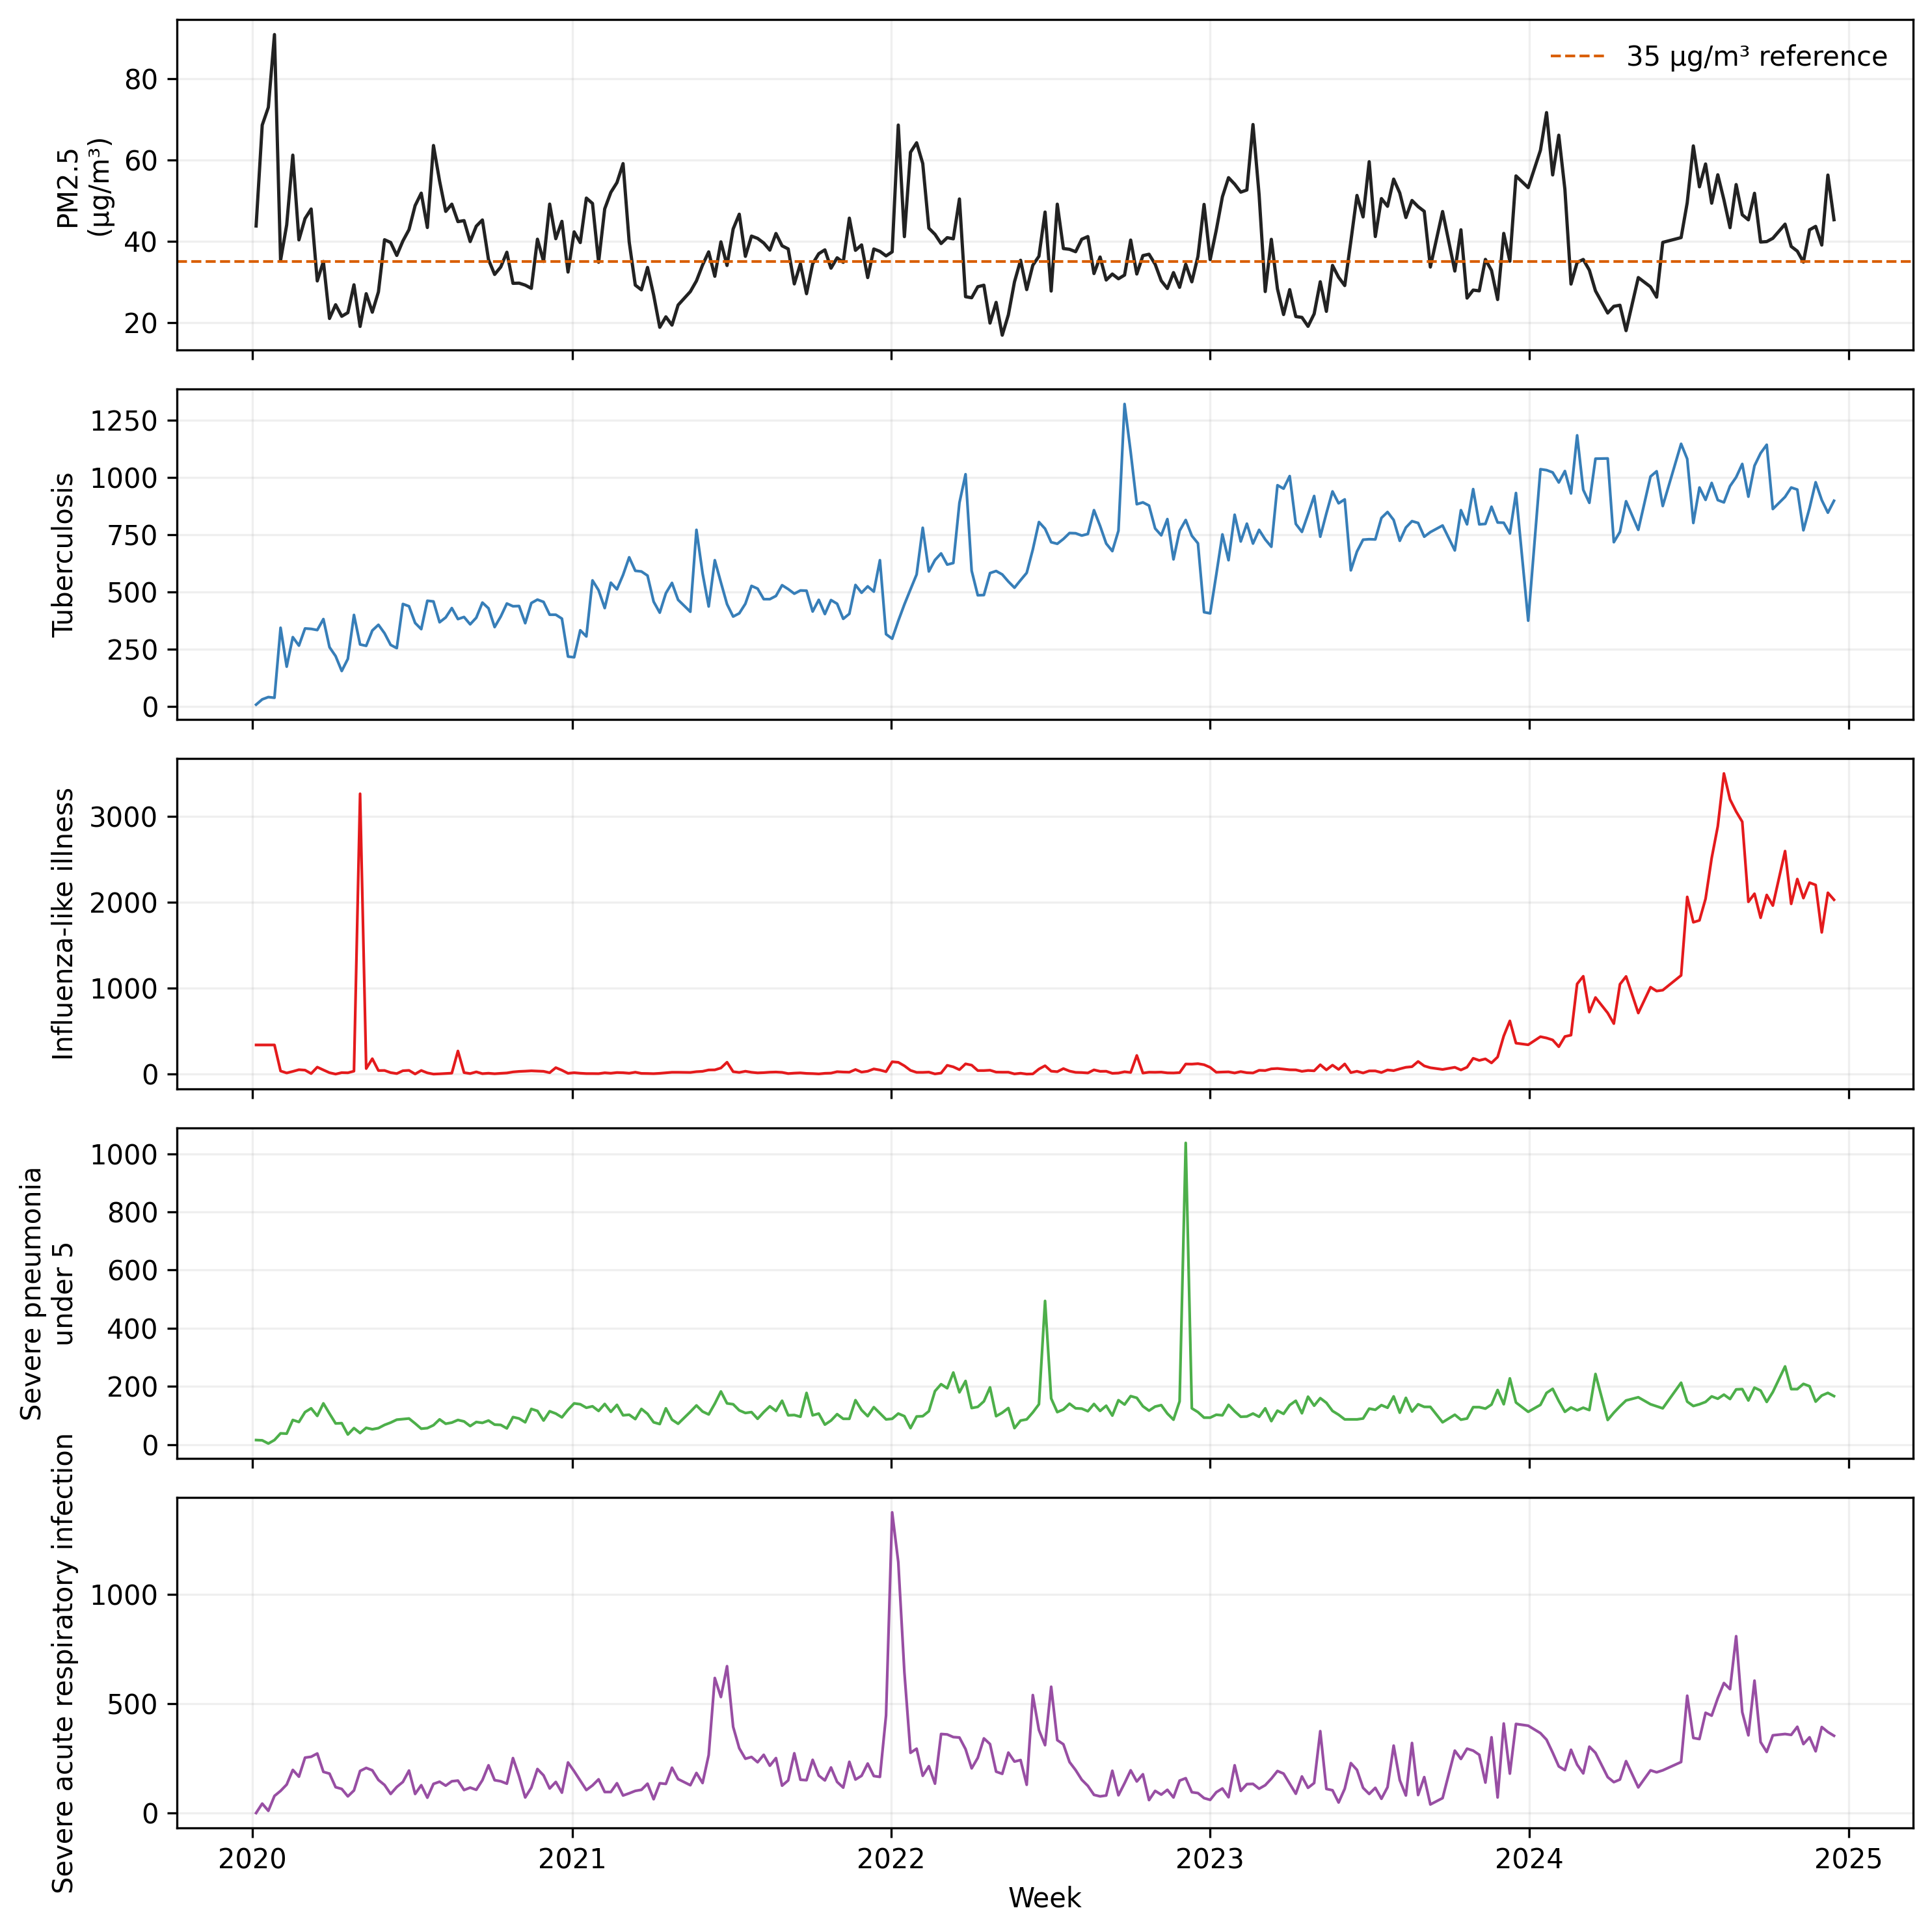
\includegraphics[width=\textwidth]{figures/time_series_overview.png}
\caption{Weekly \pmfive{} concentrations and respiratory notification counts. The dashed line is the notebook's 35 \ugm{} visual reference, not a causal threshold used in modeling.}
\label{fig:timeseries}
\end{figure}

\section{Primary adjusted associations}
ILI was the only outcome with a positive association whose 95\% CI excluded the null (Table~\ref{tab:primary}; Figure~\ref{fig:primary}). A 10 \ugm{} higher \pmfive{} concentration was associated with 17.3\% higher ILI notification counts. The estimate for SARI was positive but imprecise. The under-five pneumonia estimate was below one but compatible with the null. The inverse TB estimate was statistically precise but biologically and methodologically ambiguous; it must not be interpreted as evidence that particulate pollution protects against TB.

\begin{table}[htbp]
\centering
\caption{Primary adjusted Poisson-model associations per 10 \ugm{} higher \pmfive{}.}
\label{tab:primary}
\begin{tabular}{lrrrr}
\toprule
Outcome & IRR & 95\% CI & $p$ value & AIC \\
\midrule
TB & 0.952 & 0.924--0.981 & 0.001 & 9616.2 \\
ILI & 1.173 & 1.030--1.335 & 0.016 & 85163.4 \\
Severe pneumonia, under 5 & 0.956 & 0.908--1.005 & 0.080 & 7043.4 \\
SARI & 1.038 & 0.950--1.135 & 0.410 & 20987.4 \\
\bottomrule
\end{tabular}
\begin{flushleft}\footnotesize
All models used 248 weeks and adjusted for temperature, relative humidity, precipitation, calendar month, and linear time. HC3 robust standard errors were used.
\end{flushleft}
\end{table}

\begin{figure}[htbp]
\centering
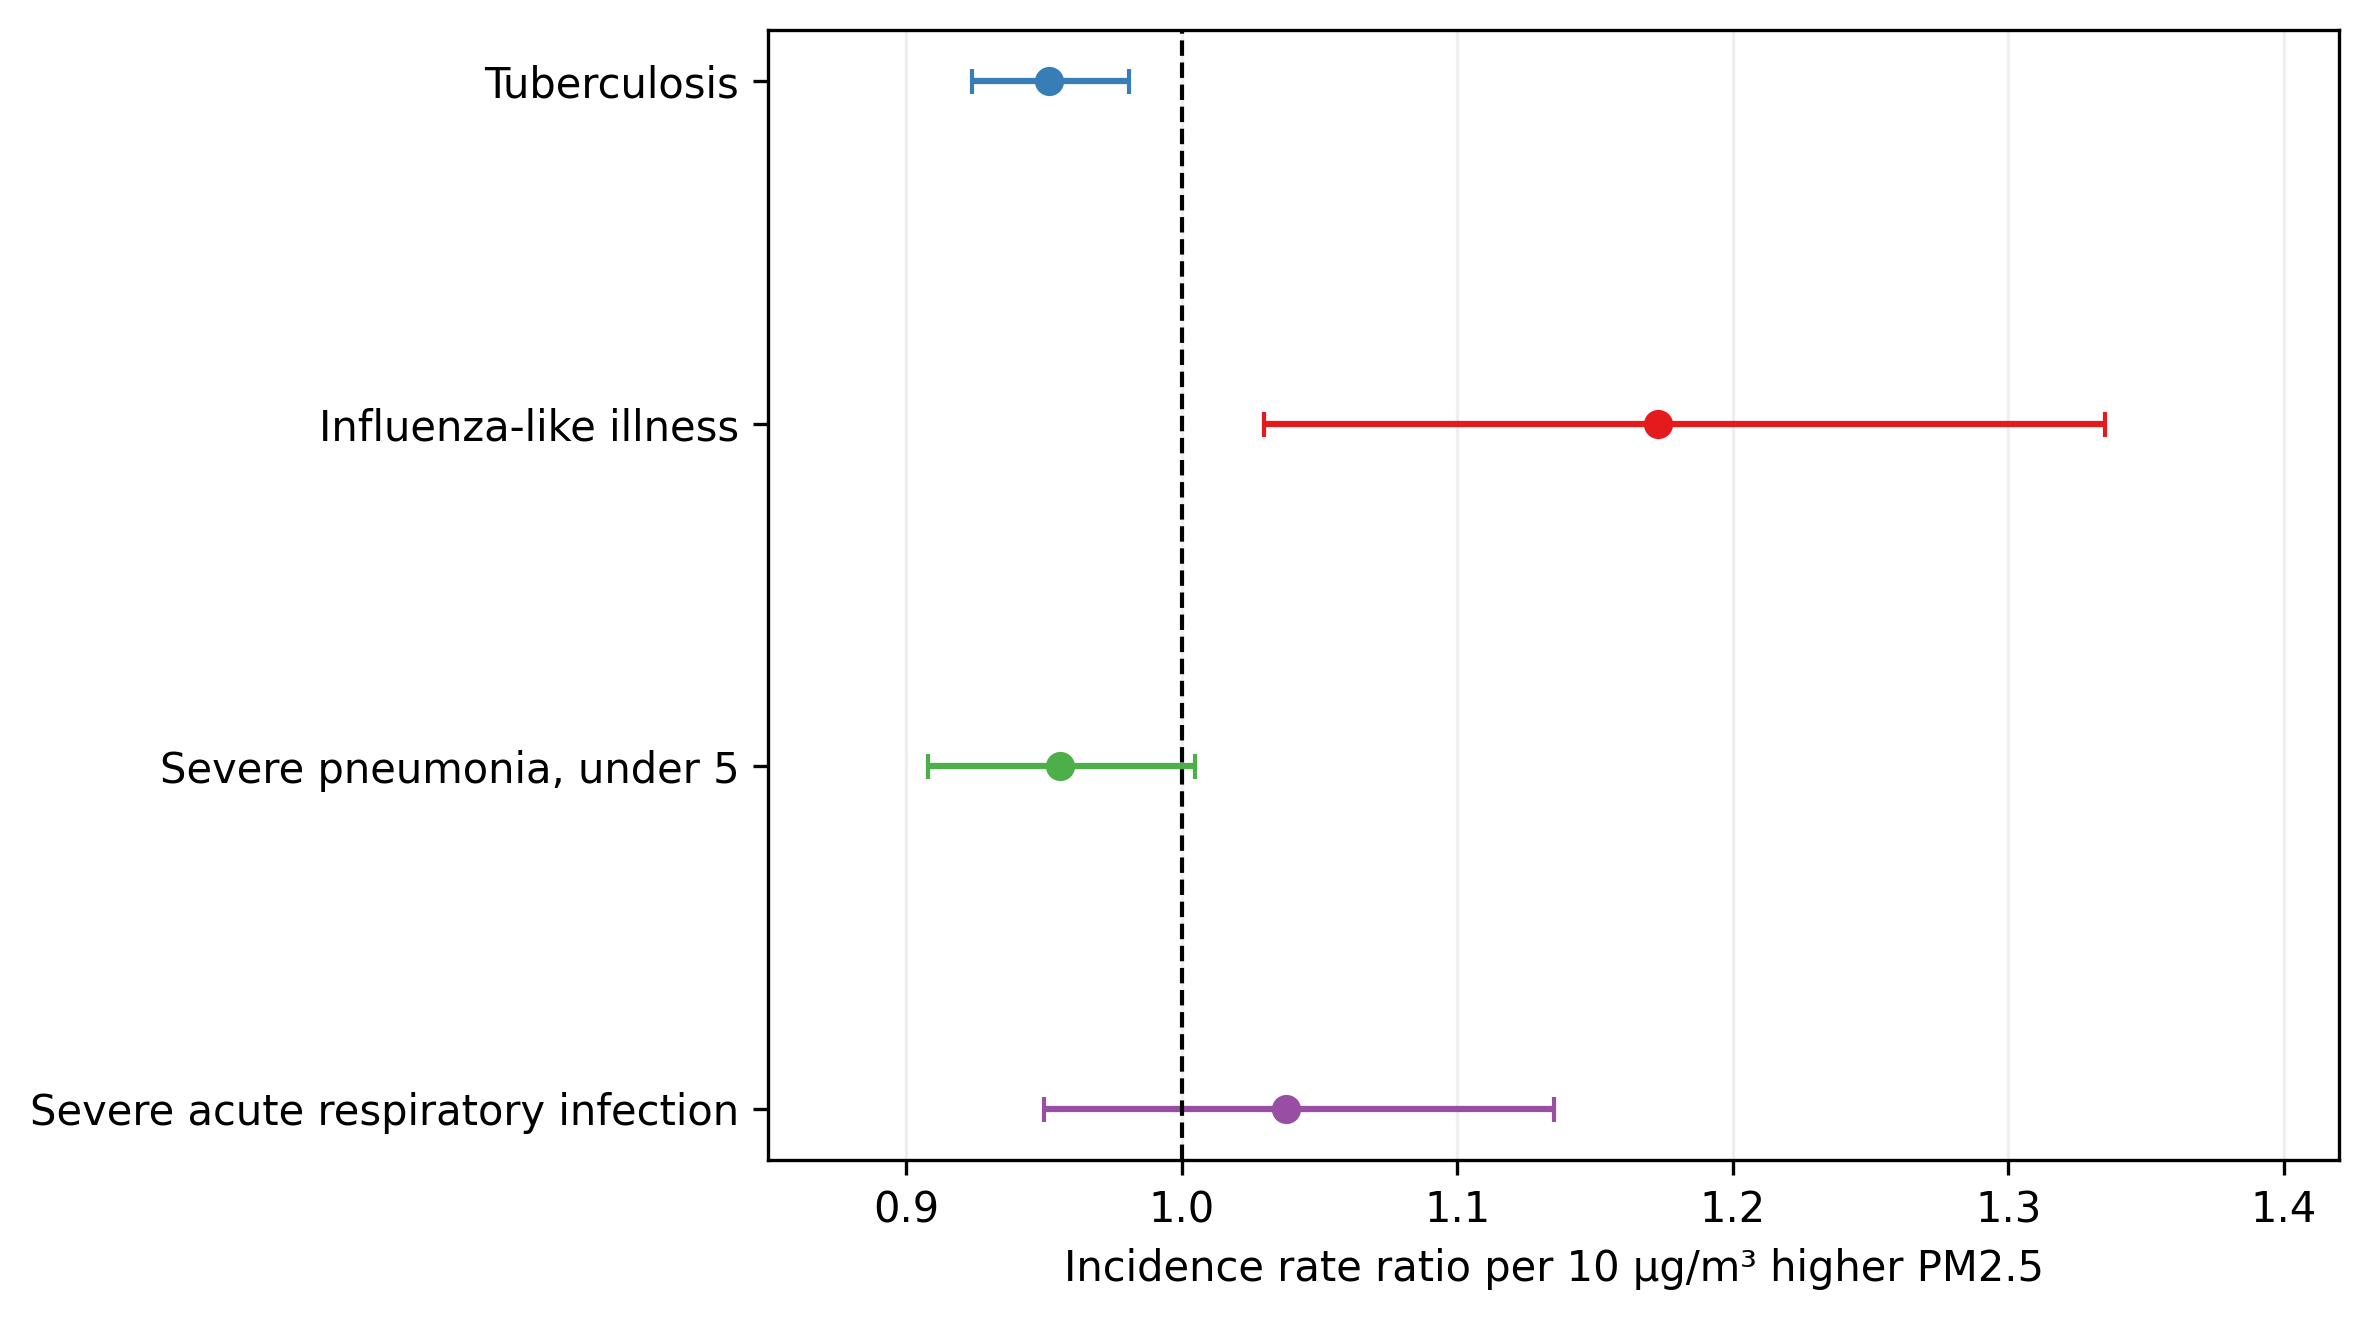
\includegraphics[width=0.88\textwidth]{figures/adjusted_irr_forest.png}
\caption{Primary adjusted incidence rate ratios. Points are IRRs per 10 \ugm{} higher \pmfive{}; horizontal bars are 95\% confidence intervals.}
\label{fig:primary}
\end{figure}

\section{Lagged and climate associations}
The 0--4-week cumulative association was positive for ILI (IRR 1.192, 95\% CI 1.032--1.377) and was compatible with the null for TB (0.977, 0.952--1.002), severe pneumonia (0.969, 0.903--1.039), and SARI (1.043, 0.951--1.144) (Figure~\ref{fig:lag}). No single lag pattern by itself supplies strong evidence of a consistent exposure response for every outcome.

The harmonised, non-imputed weekly sensitivity analysis used 262 environmental weeks and estimated all five lags jointly. It found a positive ILI association at one-week lag (IRR 1.327, 95\% CI 1.086--1.621) and a borderline positive association at four-week lag (1.220, 1.000--1.487). The corresponding monthly analysis found positive ILI associations at lag 0 (1.836, 1.326--2.543) and lag 2 (2.421, 1.533--3.824), and a positive SARI association at two-month lag (1.546, 1.288--1.856). Several inverse lag estimates were also observed, including under-five pneumonia at weekly lag 2 (0.934, 0.885--0.985) and TB at weekly lag 4 (0.956, 0.931--0.981). Given the multiple lags, small effective samples for some outcomes, and changing signs across lags, these are exploratory sensitivity findings rather than confirmatory effects.

\begin{figure}[htbp]
\centering
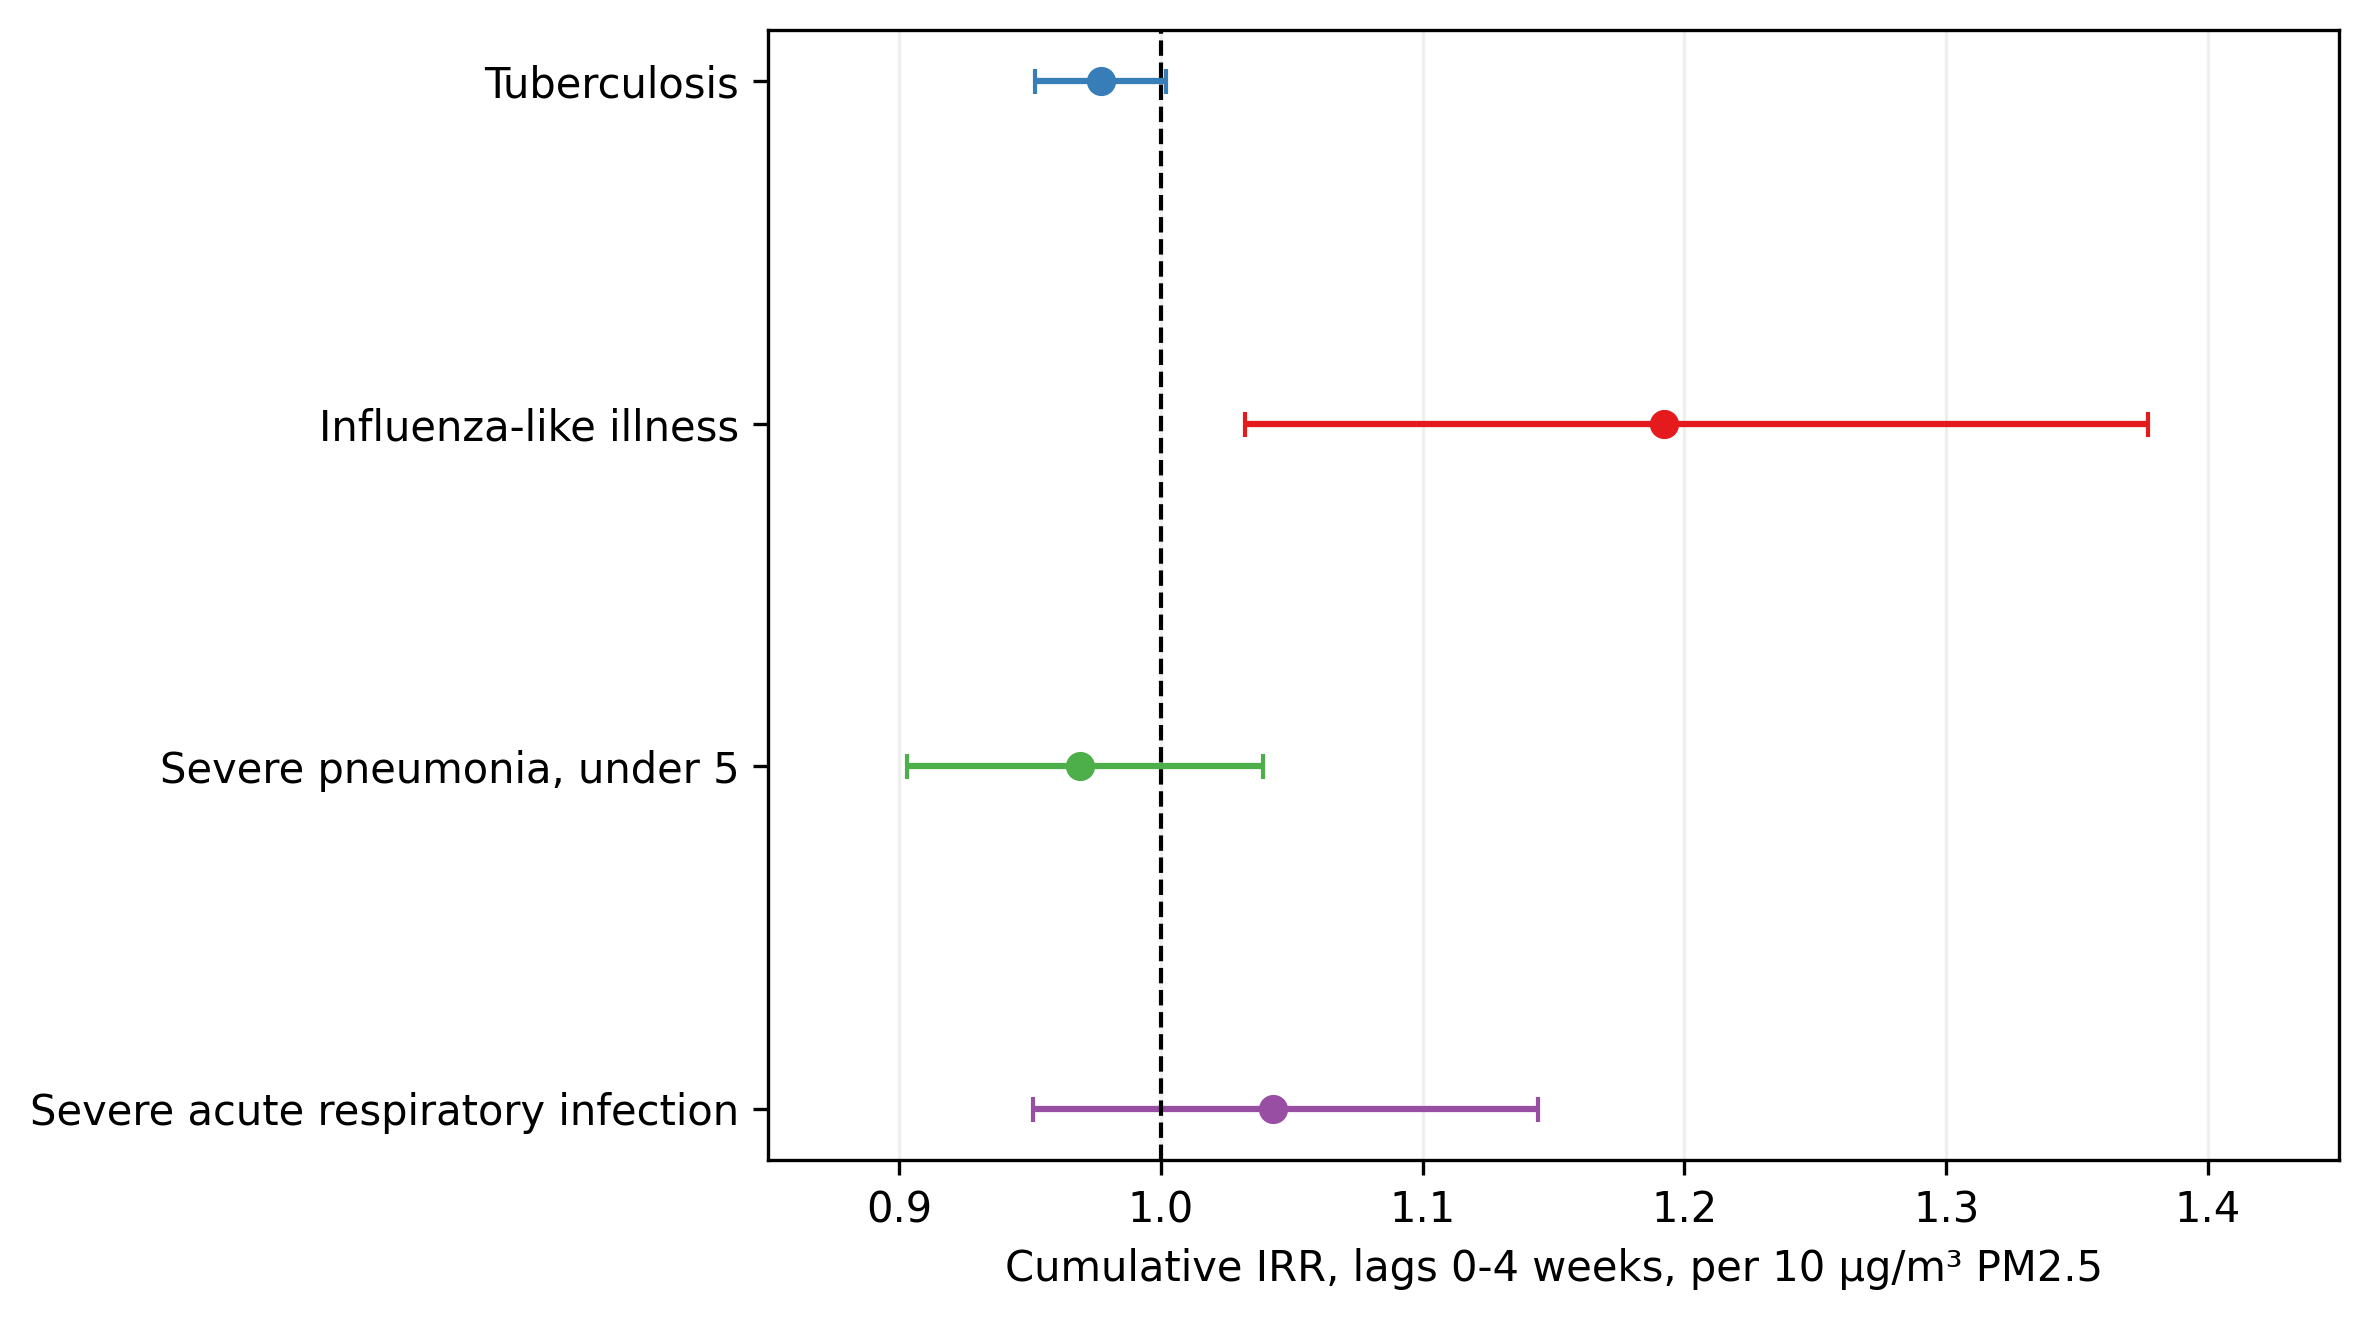
\includegraphics[width=0.88\textwidth]{figures/distributed_lag_forest.png}
\caption{Cumulative 0--4-week adjusted lag associations per 10 \ugm{} higher \pmfive{}.}
\label{fig:lag}
\end{figure}

Temperature was inversely associated with TB notifications (IRR 0.945 per 1$^\circ$C, 95\% CI 0.909--0.983; $p=0.005$). All other temperature and humidity estimates were imprecise at the 0.05 level. This pattern reinforces that weather and time-varying system factors are important potential confounders and not merely nuisance covariates.

\section{Seasonal and spatial patterns}
Seasonal profiles varied by outcome (Figure~\ref{fig:season}). In the notebook's seasonal totals, ILI and SARI notifications were highest during June--August, whereas under-five severe pneumonia had its largest total in December. Such temporal structure motivates adjustment for month but cannot eliminate residual seasonal confounding.

The legacy descriptive monitor export showed division-level monitored means from 32.26 \ugm{} in Nakawa to 54.33 \ugm{} in Rubaga (Figure~\ref{fig:map}). In the temporally linked medical-record panel, division mean exposures ranged from 32.26 \ugm{} in Nakawa to 58.96 \ugm{} in Rubaga. The linked panel included 5,006 eligible records, of which 3,632 had same-day division \pmfive{} assignment; monitoring density varied from one to 2.46 mean active sites by division. The largest number of linked records was in Rubaga (1,175), followed by Nakawa (1,077) and Makindye (953). These quantities reflect the reviewed facility record source and its residence reporting, not community disease incidence.

In weekly division--time rate models, within-division PM variation was not estimated precisely for ILI (IRR 1.090 per 10 \ugm{}, 95\% CI 0.966--1.230), pneumonia (1.060, 0.995--1.128), severe acute respiratory infection (0.958, 0.864--1.062), or TB (1.001, 0.978--1.024). The small severe-pneumonia stratum was not modelled. In the secondary diagnosis case-mix analysis, higher \pmfive{} was associated with higher odds of ILI versus the other reviewed diagnoses (OR 1.749, 1.490--2.053) and lower odds of TB (0.848, 0.779--0.923). These case-mix associations do not estimate occurrence of RTI in the population and should not be interpreted as causal or as substitutes for the rate models.

\begin{table}[htbp]
\centering
\caption{Updated weekly division-level recorded-case rate models, 2020--2024. Estimates are within-division IRRs per 10 \ugm{} higher \pmfive{}.}
\label{tab:spatial-rate}
\begin{tabular}{lrrr}
\toprule
Diagnosis & $N$ strata & IRR & 95\% CI \\
\midrule
Influenza-like illness & 85 & 1.090 & 0.966--1.230 \\
Pneumonia & 173 & 1.060 & 0.995--1.128 \\
Severe acute respiratory infection & 78 & 0.958 & 0.864--1.062 \\
Tuberculosis & 1,332 & 1.001 & 0.978--1.024 \\
Severe pneumonia & 14 & \multicolumn{2}{c}{Insufficient data} \\
\bottomrule
\end{tabular}
\begin{flushleft}\footnotesize
Counts were grouped by division, week, sex, age band, and diagnosis. Models used approximate population offsets and adjusted for division mean \pmfive{}, calendar month, linear time, sex, and age band.
\end{flushleft}
\end{table}

\begin{figure}[htbp]
\centering
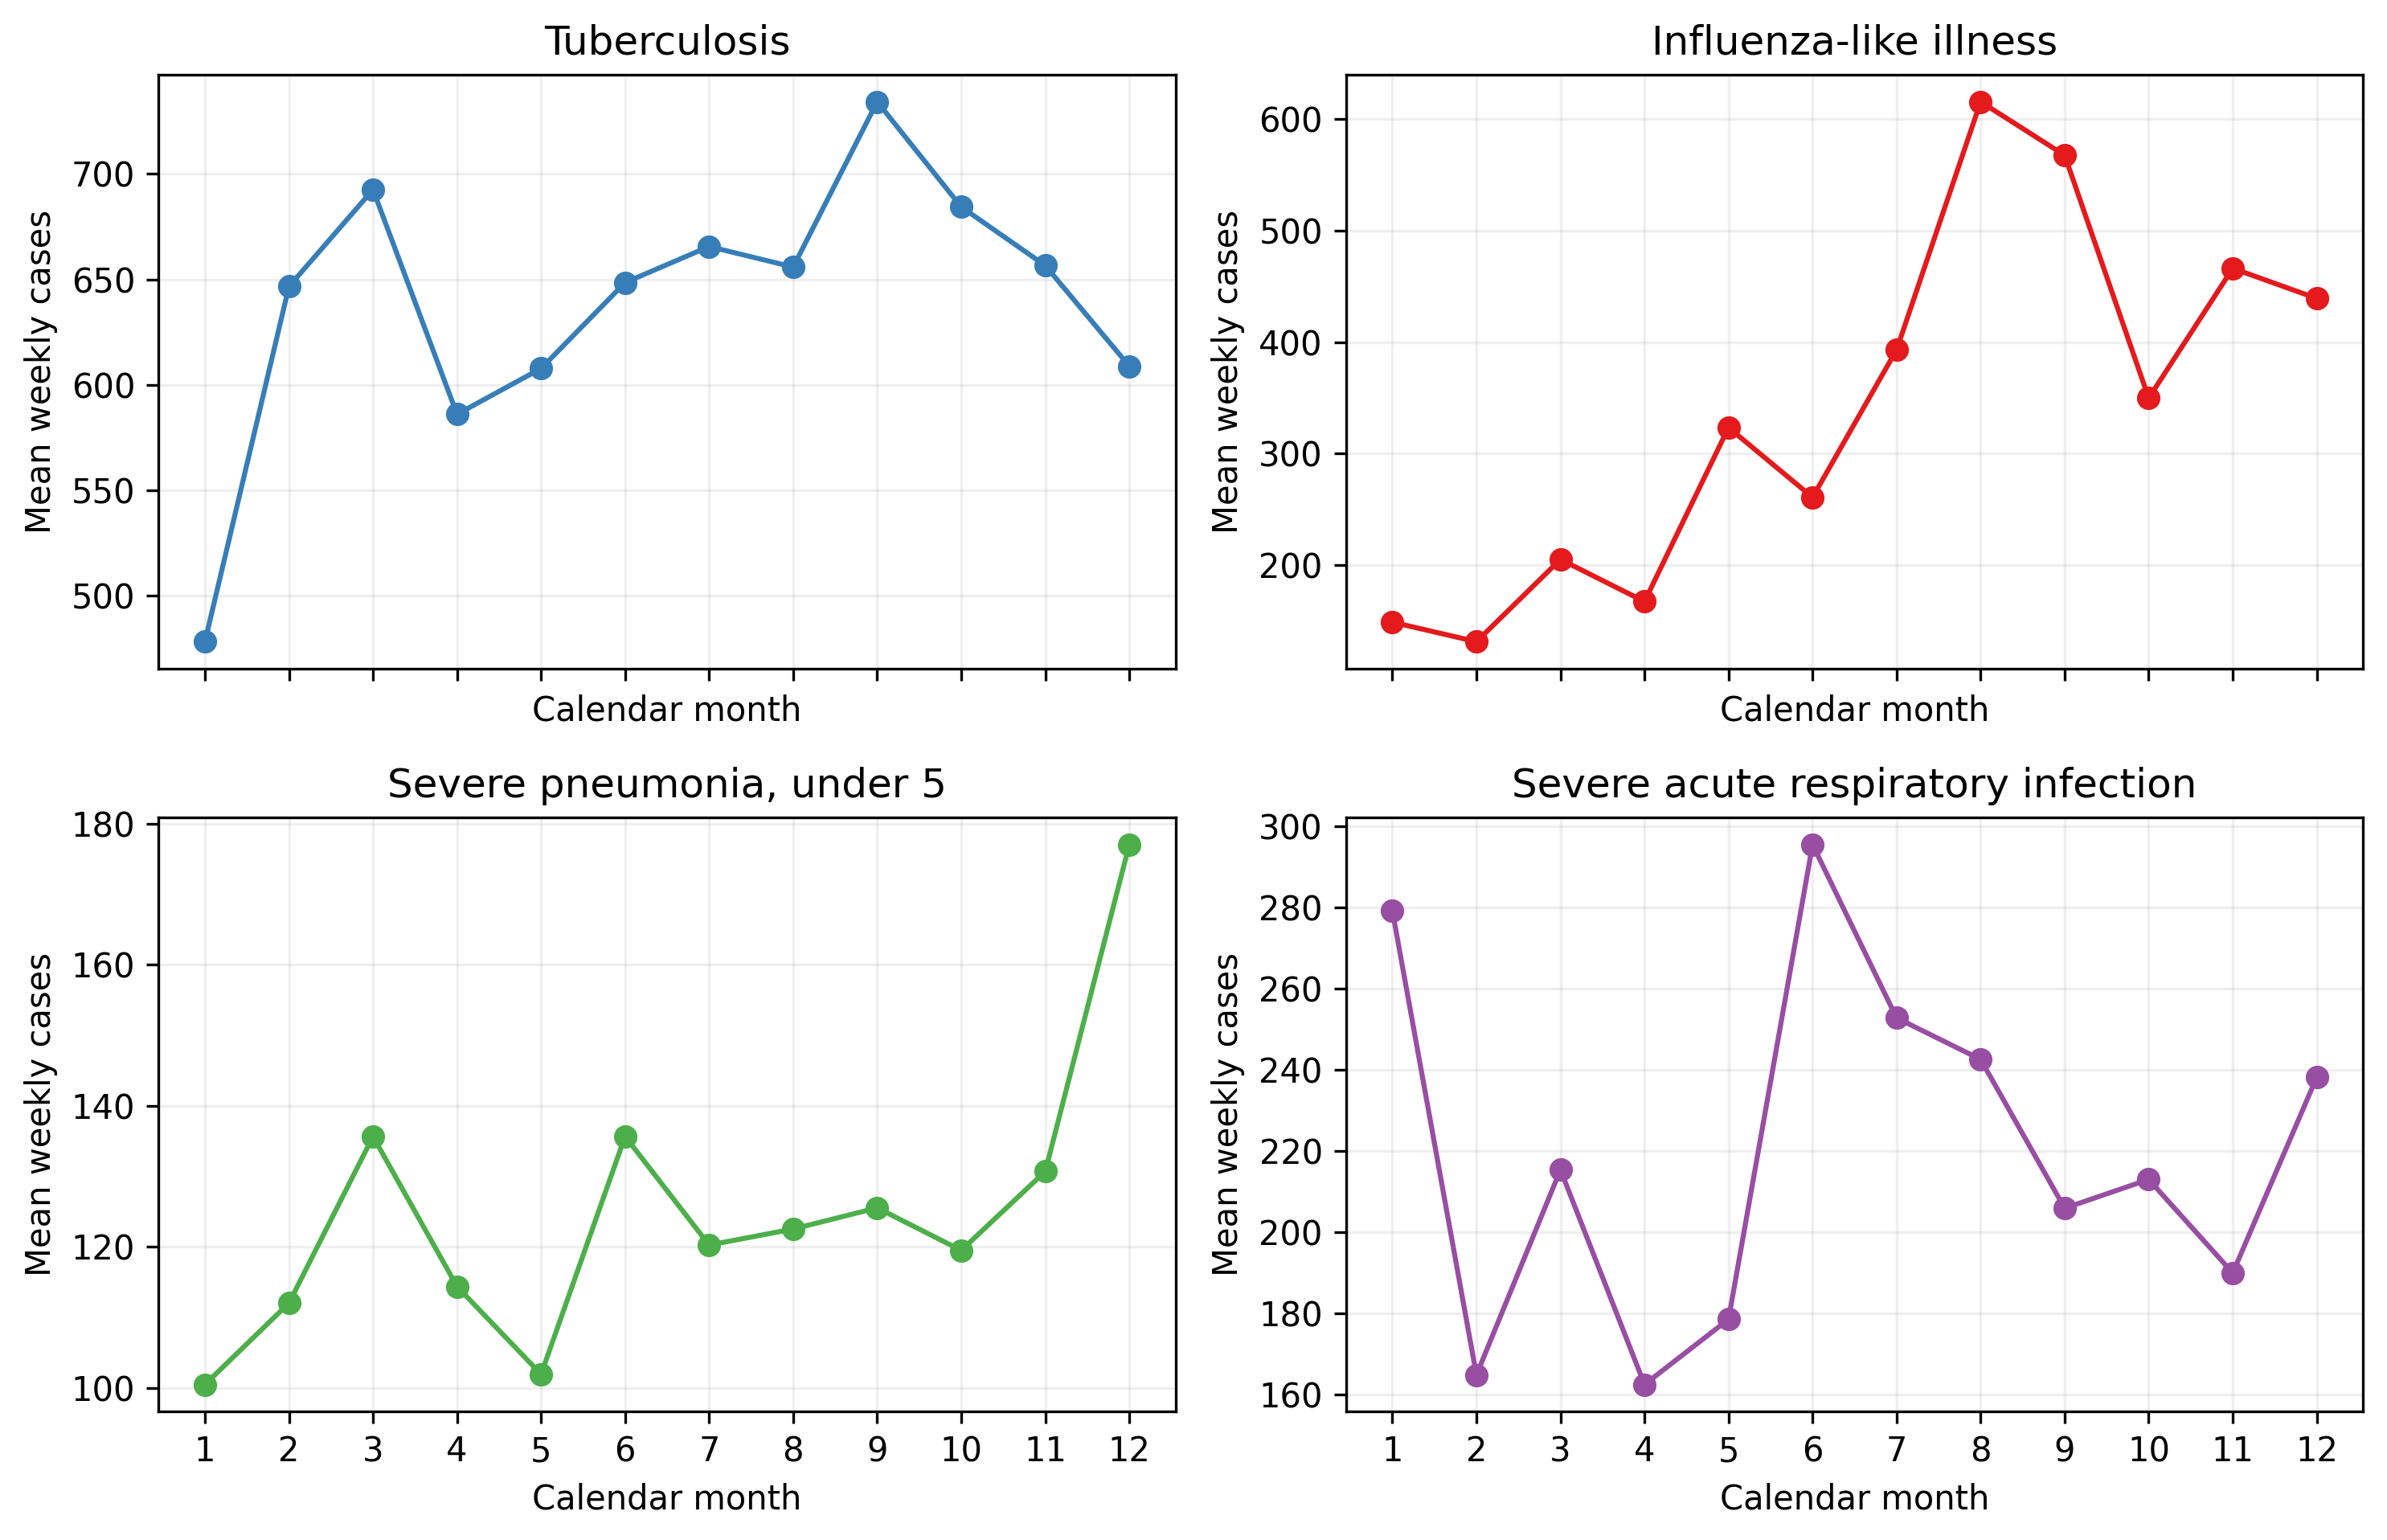
\includegraphics[width=\textwidth]{figures/seasonal_patterns.png}
\caption{Mean weekly notifications by calendar month. Each panel has its own outcome scale.}
\label{fig:season}
\end{figure}

\begin{figure}[htbp]
\centering
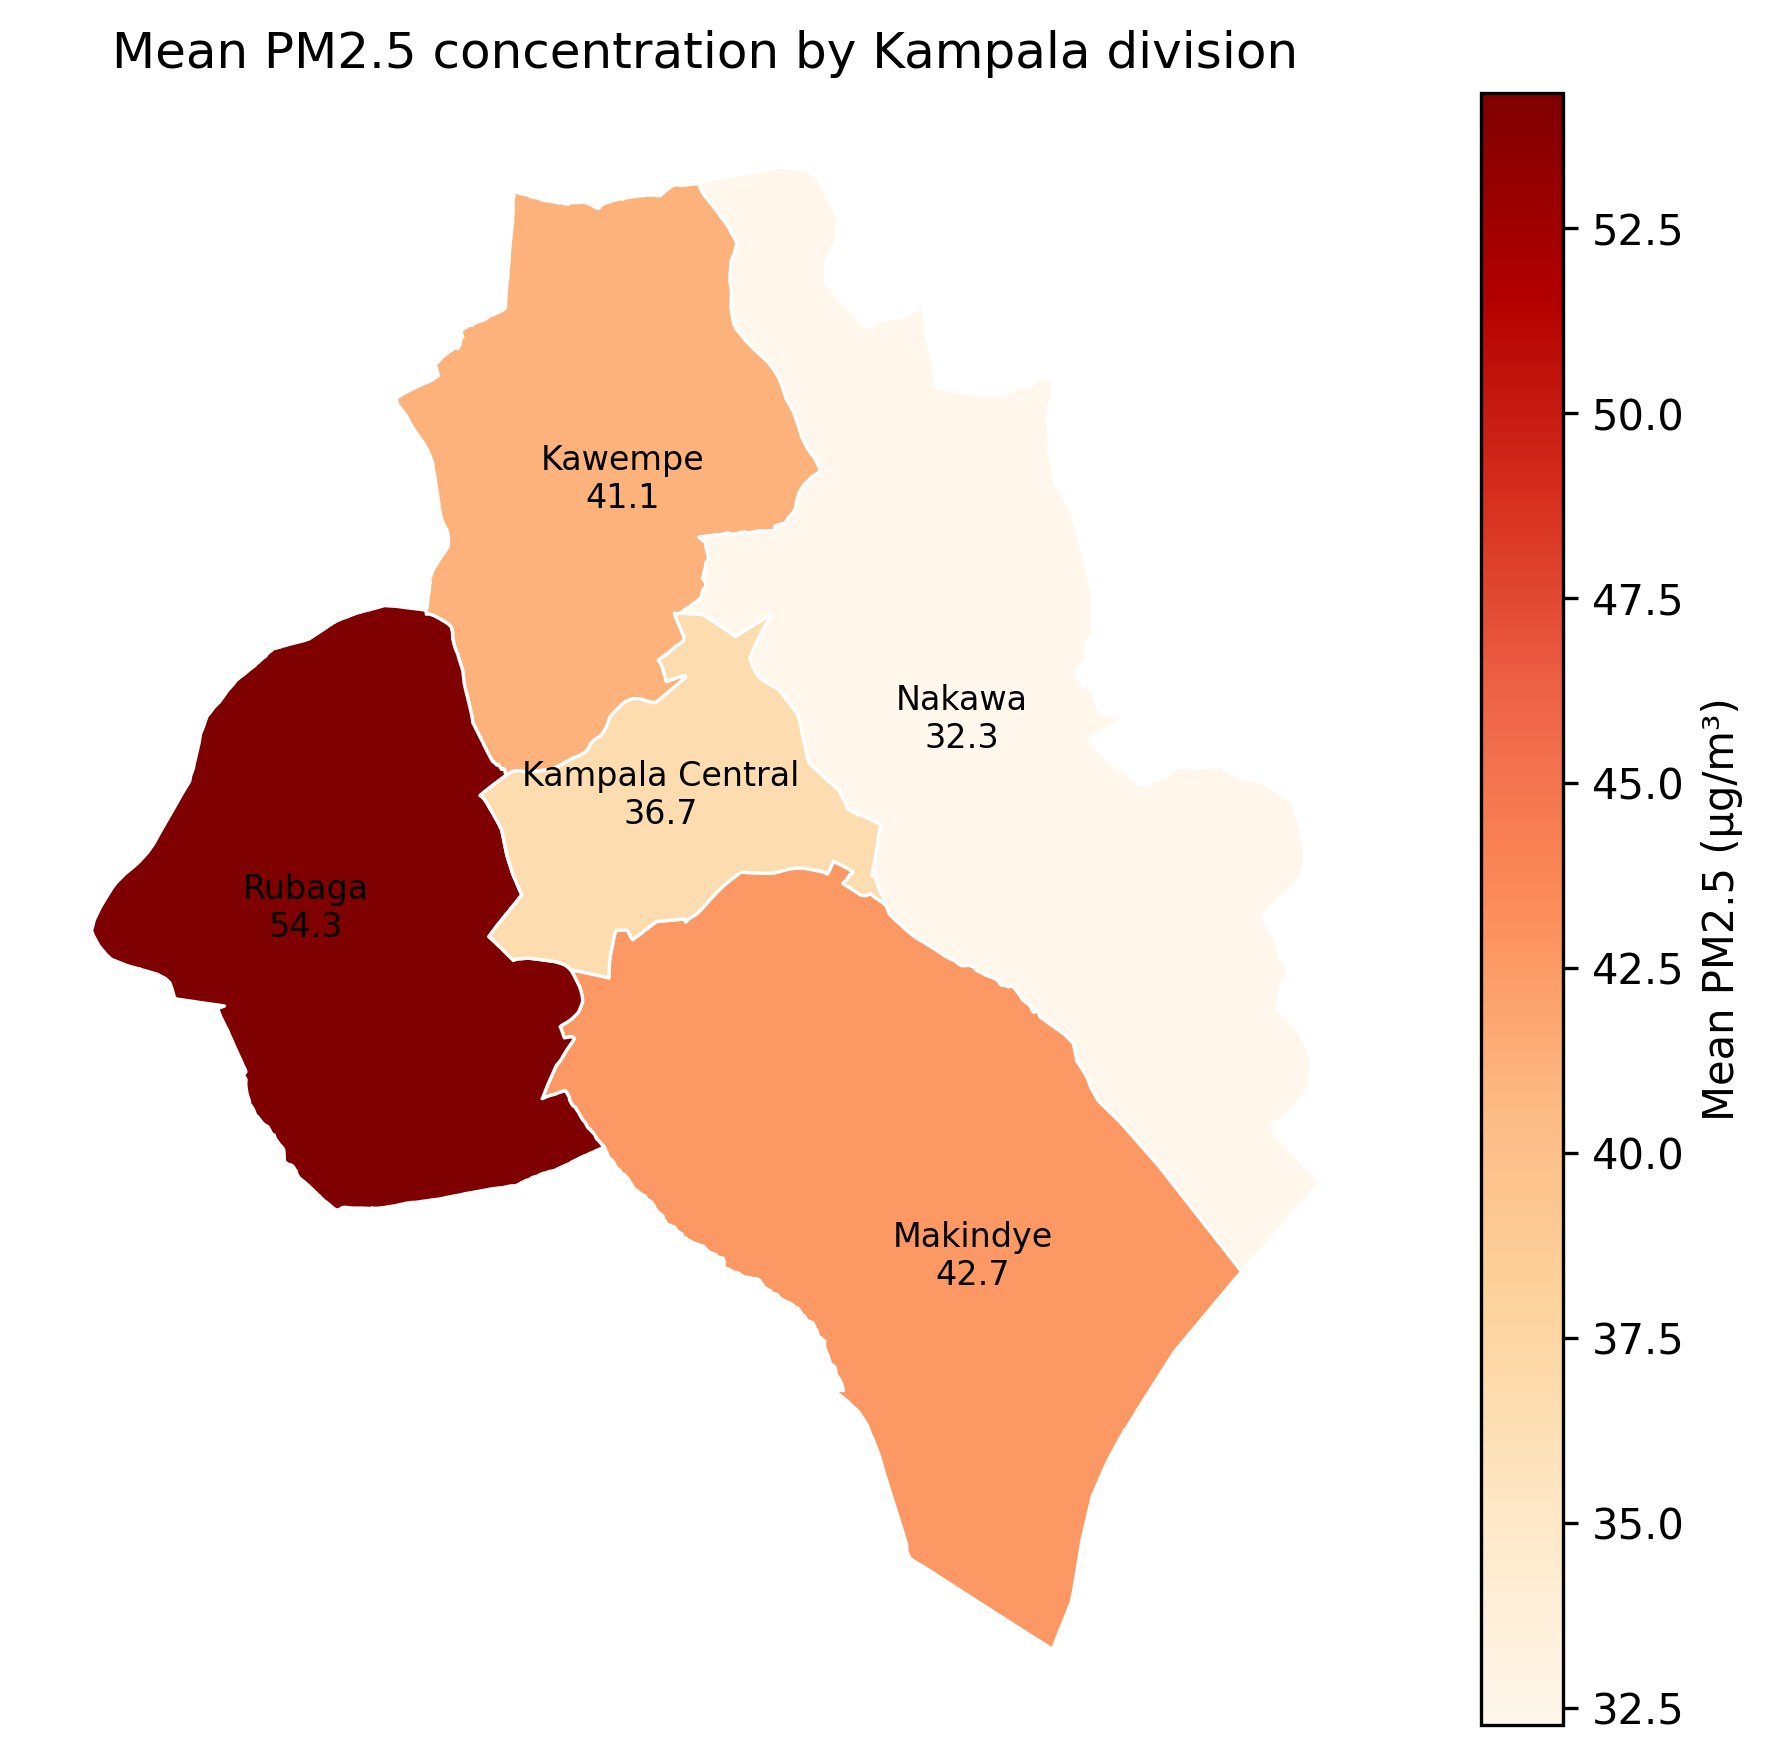
\includegraphics[width=0.72\textwidth]{figures/kampala_pm25_map.png}
\caption{Mean monitored \pmfive{} concentration by Kampala division in the supplied spatial monitor exports.}
\label{fig:map}
\end{figure}

\section{Sensitivity analysis}
The positive ILI association changed little in both sensitivity analyses (Table~\ref{tab:sensitivity}). The TB association attenuated toward the null with a one-week exposure lag. The remaining outcomes remained non-significant. These checks demonstrate some within-notebook stability but do not resolve structural biases in exposure measurement, diagnostics, reporting, or unmeasured confounding.

\begin{table}[htbp]
\centering
\caption{Sensitivity analyses for \pmfive{} associations, IRR per 10 \ugm{} higher exposure.}
\label{tab:sensitivity}
\begin{tabular}{llrrr}
\toprule
Outcome & Specification & $N$ & IRR & 95\% CI \\
\midrule
TB & Primary & 248 & 0.952 & 0.924--0.981 \\
TB & Exclude highest 5\% & 235 & 0.967 & 0.941--0.994 \\
TB & One-week lag & 247 & 0.978 & 0.955--1.002 \\
ILI & Primary & 248 & 1.173 & 1.030--1.335 \\
ILI & Exclude highest 5\% & 235 & 1.171 & 1.023--1.341 \\
ILI & One-week lag & 247 & 1.171 & 1.020--1.344 \\
Pneumonia, under 5 & Primary & 248 & 0.956 & 0.908--1.005 \\
Pneumonia, under 5 & Exclude highest 5\% & 235 & 0.981 & 0.915--1.051 \\
Pneumonia, under 5 & One-week lag & 247 & 0.961 & 0.904--1.022 \\
SARI & Primary & 248 & 1.038 & 0.950--1.135 \\
SARI & Exclude highest 5\% & 235 & 1.044 & 0.962--1.133 \\
SARI & One-week lag & 247 & 1.007 & 0.939--1.081 \\
\bottomrule
\end{tabular}
\end{table}

\chapter{Discussion}
\section{Interpretation}
The legacy primary analysis identified a positive association between weekly \pmfive{} and ILI notifications, supported by its cumulative-lag and original sensitivity results. The harmonised re-analysis retained positive ILI estimates at selected weekly and monthly lags, but the direction and precision varied across lags and outcomes. The division-level recorded-case rate model did not provide precise evidence of a within-division \pmfive{} association for ILI. Taken together, the findings are compatible with a possible short-term association but are not internally uniform enough to support a causal conclusion.

The inverse TB association requires particularly cautious interpretation. TB notifications are shaped by chronic disease processes, care pathways, diagnostic capacity, treatment programs, and reporting conventions that need not respond to weekly ambient exposure in a simple way. An apparent inverse short-term ecological association can arise from residual temporal confounding, exposure misclassification, changes in services, non-comparable reporting, model misspecification, or chance. It is not a basis for a protective interpretation.

The absence of conventional statistical significance for SARI and under-five severe pneumonia is not evidence of no effect. Confidence intervals include potentially relevant positive and negative effects, while outcome ascertainment, small effective temporal variation, aggregation, and limited covariate control constrain precision and validity.

\section{Strengths}
Strengths include a multiyear weekly series, explicit linkage of environmental and surveillance sources, multiple respiratory outcomes, lag analyses, and transparent sensitivity checks. The updated work adds a non-imputed canonical time-series sensitivity pipeline, a documented medical-record selection flow, same-day division-level exposure assignment, sex- and age-stratified recorded-case rates, population denominators, and explicit reporting of unresolved parish linkage. The chapter also distinguishes exploratory analyses from primary inference and retains the complete no-mortality analytic scope.

\section{Limitations}
First, this ecological analysis cannot link personal exposure to an individual's outcome. Second, citywide or division-level averaged monitor data can misclassify individual exposure. Third, missing calendar weeks, the legacy pipeline's mean imputation, and reliance on routine notifications can introduce artifacts. Fourth, the medical-review data are facility records and not a population sample; referral, care-seeking, diagnostic practice, and facility catchment can all affect recorded counts. Fifth, only 2,425 of 5,006 eligible records had an exact or reviewed parish-to-population match, and only 3,632 had same-day division exposure; no parish-level inferential results are therefore claimed. Sixth, sex--age denominators were approximated from marginal population counts rather than observed cross-classified denominators. Finally, the simplified linear lag model does not characterize non-linear concentration-response relationships, and the spatial analysis cannot reproduce the reference study's Bayesian multilevel design because this dataset contains reviewed respiratory cases rather than sampled cases and non-cases \parencite{Adjorlolo2026}.

\section{Implications and recommendations}
Kampala should strengthen interoperable environmental and health surveillance, preserve facility-level denominators and diagnostic metadata, and maintain calibrated monitors with documented coverage. Future research should pre-specify causal estimands, use population offsets and finer spatial-temporal exposure assignment, evaluate overdispersion and autocorrelation, include non-linear splines and formal distributed-lag cross-bases, and validate findings against independent data. Pollution-reduction decisions should use the broader health evidence base and local feasibility assessments rather than the chapter's scenario calculations alone.

\chapter{Conclusion}
Across the legacy 248-week primary series and the updated 262-week canonical sensitivity series, positive \pmfive{}--ILI associations appeared in several, but not all, specifications. Associations for SARI and under-five pneumonia varied by lag, while inverse TB estimates are not plausibly interpretable as protection. The new medical-record analysis provides division, sex, age, and population-aware context but found no precise within-division rate association for the main diagnoses; its ILI case-mix association is not an individual-risk estimate. These findings are hypothesis-generating observational evidence. They justify improved surveillance, complete residence/population linkage, and more rigorous prospective analysis, not causal claims about individual risk or predicted benefits of a specific intervention.

\appendix
\chapter{Reproducibility and analytic specifications}
The primary reproducibility artifact is \texttt{analysis\_no\_deaths.ipynb}. It reads project-supplied climate, \pmfive{}, and routine respiratory data; removes all mortality outcomes; creates the merged weekly analytic file; and calculates the reported outputs. The companion script \texttt{generate\_thesis\_assets.py} regenerates the no-mortality merged input and the figures used in this chapter. Re-running the complete notebook may change stochastic neural-network outputs unless random seeds and software versions are fixed.

\chapter{Exploratory analyses}\label{app:exploratory}
\section{Interrupted time-series reference}
The notebook set 29 May 2022 (the series midpoint) as an intervention reference. No documented external intervention was identified in the supplied material. Consequently, any before--after or interrupted-time-series contrast is a synthetic modeling reference and is not reported as an intervention effect.

\section{Forecasting diagnostics}
The fusion LSTM model used 188 training and 48 test samples for each outcome. Its out-of-sample performance was poor: TB RMSE 364.25 and $R^2=-6.09$; ILI RMSE 1721.38 and $R^2=-2.71$; under-five severe pneumonia RMSE 287.34 and $R^2=-61.21$; and SARI RMSE 310.67 and $R^2=-3.76$. Negative $R^2$ values show that these configurations performed worse than a mean-baseline benchmark on the test data. They are not suitable for operational forecasting without redesign, tuning, external validation, and uncertainty evaluation.

\section{Scenario calculations}
The notebook considered 15\%, 20\%, 25\%, and 35\% hypothetical \pmfive{} reductions and calculated expected prevented cases using a fixed assumed relative risk of 1.08 per 10 \ugm{} change. This assumption was not estimated separately for each outcome in the primary models and ignores uncertainty, feasibility, costs, exposure distributions, and causal identification. The calculations should therefore be treated as illustrative arithmetic, not policy-effect estimates.

\printbibliography
\end{document}
